\documentclass[english,man,floatsintext,draftall]{apa6}
\usepackage{lmodern}
\usepackage{amssymb,amsmath}
\usepackage{ifxetex,ifluatex}
\usepackage{fixltx2e} % provides \textsubscript
\ifnum 0\ifxetex 1\fi\ifluatex 1\fi=0 % if pdftex
  \usepackage[T1]{fontenc}
  \usepackage[utf8]{inputenc}
\else % if luatex or xelatex
  \ifxetex
    \usepackage{mathspec}
  \else
    \usepackage{fontspec}
  \fi
  \defaultfontfeatures{Ligatures=TeX,Scale=MatchLowercase}
\fi
% use upquote if available, for straight quotes in verbatim environments
\IfFileExists{upquote.sty}{\usepackage{upquote}}{}
% use microtype if available
\IfFileExists{microtype.sty}{%
\usepackage{microtype}
\UseMicrotypeSet[protrusion]{basicmath} % disable protrusion for tt fonts
}{}
\usepackage[unicode=true]{hyperref}
\hypersetup{
            pdftitle={Postural developments modulate children's visual access to social information},
            pdfkeywords={Postural developments modulate children's visual access to social
information},
            pdfborder={0 0 0},
            breaklinks=true}
\urlstyle{same}  % don't use monospace font for urls
\ifnum 0\ifxetex 1\fi\ifluatex 1\fi=0 % if pdftex
  \usepackage[shorthands=off,main=english]{babel}
\else
  \usepackage{polyglossia}
  \setmainlanguage[]{english}
\fi
\usepackage{graphicx,grffile}
\makeatletter
\def\maxwidth{\ifdim\Gin@nat@width>\linewidth\linewidth\else\Gin@nat@width\fi}
\def\maxheight{\ifdim\Gin@nat@height>\textheight\textheight\else\Gin@nat@height\fi}
\makeatother
% Scale images if necessary, so that they will not overflow the page
% margins by default, and it is still possible to overwrite the defaults
% using explicit options in \includegraphics[width, height, ...]{}
\setkeys{Gin}{width=\maxwidth,height=\maxheight,keepaspectratio}
\IfFileExists{parskip.sty}{%
\usepackage{parskip}
}{% else
\setlength{\parindent}{0pt}
\setlength{\parskip}{6pt plus 2pt minus 1pt}
}
\setlength{\emergencystretch}{3em}  % prevent overfull lines
\providecommand{\tightlist}{%
  \setlength{\itemsep}{0pt}\setlength{\parskip}{0pt}}
\setcounter{secnumdepth}{0}
% Manuscript styling
\usepackage{upgreek}
\captionsetup{font=singlespacing,justification=justified}

% Table formatting
\usepackage{longtable}
\usepackage{lscape}
% \usepackage[counterclockwise]{rotating}   % Landscape page setup for large tables
\usepackage{multirow}		% Table styling
\usepackage{tabularx}		% Control Column width
\usepackage[flushleft]{threeparttable}	% Allows for three part tables with a specified notes section
\usepackage{threeparttablex}            % Lets threeparttable work with longtable

% Create new environments so endfloat can handle them
% \newenvironment{ltable}
%   {\begin{landscape}\begin{center}\begin{threeparttable}}
%   {\end{threeparttable}\end{center}\end{landscape}}
\newenvironment{lltable}{\begin{landscape}\begin{center}\begin{ThreePartTable}}{\end{ThreePartTable}\end{center}\end{landscape}}

% Enables adjusting longtable caption width to table width
% Solution found at http://golatex.de/longtable-mit-caption-so-breit-wie-die-tabelle-t15767.html
\makeatletter
\newcommand\LastLTentrywidth{1em}
\newlength\longtablewidth
\setlength{\longtablewidth}{1in}
\newcommand{\getlongtablewidth}{\begingroup \ifcsname LT@\roman{LT@tables}\endcsname \global\longtablewidth=0pt \renewcommand{\LT@entry}[2]{\global\advance\longtablewidth by ##2\relax\gdef\LastLTentrywidth{##2}}\@nameuse{LT@\roman{LT@tables}} \fi \endgroup}

% \setlength{\parindent}{0.5in}
% \setlength{\parskip}{0pt plus 0pt minus 0pt}

% \usepackage{etoolbox}
\makeatletter
\patchcmd{\HyOrg@maketitle}
  {\section{\normalfont\normalsize\abstractname}}
  {\section*{\normalfont\normalsize\abstractname}}
  {}{\typeout{Failed to patch abstract.}}
\makeatother
\shorttitle{Posture modulates social access}
\author{Bria L. Long\textsuperscript{1}, Alessandro Sanchez\textsuperscript{1}, Allison M. Kraus\textsuperscript{1}, Ketan Agrawal\textsuperscript{1}, \& Michael C. Frank\textsuperscript{1}}
\affiliation{
\vspace{0.5cm}
\textsuperscript{1} Department of Psychology, Stanford University}
\authornote{

Correspondence concerning this article should be addressed to Bria L. Long, 450 Serra Mall, Stanford CA 94305. E-mail: bria@stanford.edu}
\keywords{Postural developments modulate children's visual access to social information\newline\indent Word count: X}
\usepackage{lineno}

\linenumbers
\usepackage{csquotes}

\title{Postural developments modulate children's visual access to social
information}

\date{}

\abstract{
The ability to process social information is a critical component of
children's early language and cognitive development. However, as
children reach their first birthday, they begin to locomote themselves,
dramatically affecting their visual access to this information. How do
these postural and locomotor changes affect children's access to the
social information relevant for word-learning? Here, we explore this
question by using head-mounted cameras to record 36 infants' (8-16
months of age) egocentric visual perspective and use computer vision
algorithms to estimate the proportion of faces and hands in infants'
environments. We find that infants' posture and orientation to their
caregiver modulates their access to social information, confirming
previous work that suggests motoric developments play a significant role
in the emergence of children's linguistic and social capacities. In
addition, we applied our automated analysis to the headcam data from a
recent paper showing similar effects postre on visual attention
(Franchak et al., 2017), finding convergence across methodologies,
laboratories, and datasets. We suggest that the combined use of
head-mounted cameras and the application of new computer vision
techniques is a promising avenue for understanding the statistics of
infants' visual and linguistic experience as they change over
development.
}

\begin{document}
\maketitle

From their earliest months, infants are deeply engaged in learning from
others. Even newborns tend to prefer to look at faces with direct
vs.~averted gaze (Farroni, Csibra, Simion, \& Johnson, 2002) and young
infants follow overt gaze shifts. And as infants learn to parse and
segment their native language(s), the social cues provided by speakers
(e.g., eye-gaze) may provide strong scaffolding for early word learning.
Indeed, empirical work suggests that children's ability to process
social cues is a key factor in early language development: in a
longitudinal study, children's level of joint engagement with their
mother at 9-12 months was found to predict both their receptive and
productive vocabularies (Carpenter, Nagell, \& Tomasello, 1998). More
specifically, 10 month-olds who follow an adult's gaze in an
experimental context have larger vocabularies at 18 months and
throughout the second year of life (R. Brooks \& Meltzoff, 2005; Rechele
Brooks \& Meltzoff, 2008).

Around their first birthday, however, children's ability to interact
with their world radically changes (Adolph \& Berger, 2006) as they are
no longer constrained to the same spot that their caregivers last placed
them in. Before the first birthday, children often begin crawling; soon
after, they begin to walk independently. While not all children crawl
({\textbf{???}})---or crawl in the same way---children tend to find
creative ways of moving (e.g., scooting) or getting others to help them
move (e.g cruising) to begin to explore their world on their own
({\textbf{???}}). And as independent agents in the world, children are
more active in the construction of their own learning environments. Yet
while toddlers do determine their own input to a much greater degree,
they spend much of their time in a world primarily populated by knees

One possibility is that these motor improvements have strong
developmental cascades, impacting children's emerging social, cognitive,
and linguistic abilities (Iverson, 2010). Indeed, these postural changes
change how children interact with their mothers; walking infants make
different kinds of object-related bids for attention from their mothers
than crawling infants, and tend to hear more action directed statements
(e.g., \enquote{open it}) (Karasik, Tamis-LeMonda, \& Adolph, 2014). In
an observational study, Walle and Campos (2014) also found that children
who were able to walk had both higher receptive and productive
vocabularies. On their account, children's ability to stand and
independently locomote may fundamentally change their ability to access
the social information (e.g., faces, gaze) relative to children who are
still crawling and sitting. In other words, the ability of walking
infants to access more detailed social information may allow infants to
learn words quicker and more efficiently, facilitating language growth.

Over the past decade, researchers have started to use egocentric,
head-mounted cameras to document the social information that infants and
children have access to across early development, and to understand the
degree to which there are substantial shifts in their viewpoints that
may have downstream developmental consequences ({\textbf{???}}). Indeed,
the infant visual perspective has proved to be both remarkably different
than the adult perspective and not easily predicted by our own
intuitions (Clerkin, Hart, Rehg, Yu, \& Smith, 2017; Franchak, Kretch,
Soska, \& Adolph, 2011, Yoshida and Smith (2008)). Over the first two
years of life, the infant viewpoint transitions from primarily
containing close up view of faces to capturing relatively restricted
views of hands paired with the objects they are acting on (Fausey,
Jayaraman, \& Smith, 2016); both computational and empirical work
suggest that this restricted viewpoint is more effective for learning
about objects and their labels than the comparable adult perspective (D.
Yurovsky, Smith, \& Yu, in press, Bambach, Crandall, Smith, and Yu
(2017)).

Here, we directly examine the role that postural developments that
infants' experience as they reach their first birthday change the social
information in the infant view. We hypothesize that children's postural
developments may be partially responsible for some of these changes in
the infant perspective. During spontaneous play, toddlers are more
likely to look at the floor while crawling than while walking (Franchak
et al., 2011), when they have full visual access to their environment
and the people in it (Kretch, Franchak, and Adolph, 2014). More
recently, when 12-month-olds ({\textbf{???}}) participated in a
free-play session with their caregivers, their own posture and as well
as their caregiver's posture influenced the proportion of time they
spent looking at the faces and bodies of their caregivers
({\textbf{???}}).

Here, we expand on these previous findings in three key ways. First,
using head-mounted cameras during a brief laboratory free-play session,
we record the visual experience of three groups of children at 8, 12,
and 16 months-of-age, covering a broad range of ages and locomotor
abilities around the first birthday; Children's posture and orientation
relative to their caregiver were also recorded from a third-person
perspective and hand-annotated. This cross-sectional design thus allows
us to directly examine the relative contributions of age vs.~postural
developments on children's visual access to social information. Second,
we use a modern computer vision algorithm for the automated detection of
faces and hands in the egocentric viewpoints of infants. In particular,
we capitalize on recent improvements in face and pose detection
algorithms (Cao, Simon, Wei, \& Sheikh, 2017; K. Zhang, Zhang, Li, \&
Qiao, 2016) to analyze the frequencies of faces and hands in the child's
visual environment, both overall and relative to naming events by their
caregivers. Use of this emerging technology allows us to annotate the
entirety of the dataset, allowing a more complete picture of the
changing infant perspective. In addition, we extend this technique to
the same dataset used in ({\textbf{???}}), replicating their main
pattern of results using this novel methodology and finding convergence
between our datasets with different play sessions, populations, and
head-mounted cameras. Finally, as parents were presented with pairs of
novel and familiar objects with their children during the play sessions,
we directly examine the availability of social signals during naming
events.

Thus, our current dataset allows us to analyze changes in the visual
access to faces and hands according to children's age, posture, and
linguistic input. We predicted that there would be differential access
to social information based on children's postural developments:
crawling infants would see fewer faces/hands because they would
primarily be looking at the ground, while walking toddlers would have
access to a richer visual landscape with greater access to the social
information in their environment. {[}language predictions?{]}

\section{Methods}\label{methods}

\subsubsection{Participants}\label{participants}

Our final sample consisted of 36 infants and children, with 12
participants in three age groups: 8 months (6 F), 12 months (7 F), and
16 months (6 F). Participants were recruited from the surrounding
community via state birth records, had no documented disabilities, and
were reported to hear at least 80 percent English at home. Demographics
and exclusion rates are given in the table below.

\begin{table}[ht]
\centering
\begin{tabular}{rrrrrr}
\hline
Group & N & \% incl. & Avg age & Avg video length (min) \\
\hline
8 mo. &   12 & 0.46 & 8.71 & 14.41 \\
12 mo. &  12 & 0.40 & 12.62 & 12.71 \\
16 mo. &  12 & 0.31 & 16.29 & 15.10\\
\hline
\end{tabular}
\end{table}

To obtain this final sample, we tested 95 children, excluding 59
children for the following reasons: 20 for technical issues related to
the headcam, 15 for failing to wear the headcam, 10 for fewer than 4
minutes of headcam footage, 5 for having multiple adults present, 5 for
missing Communicative Development Inventory (CDI) data, 2 for missing
scene camera footage, 1 for fussiness, and one for sample symmetry. All
inclusion decisions were made independent of the results of subsequent
analyses. Some of these data were also analyzed in Frank, Simmons,
Yurovsky, and Pusiol (2013).

\subsubsection{Procedure}\label{procedure}

All parents signed consent documents while children were fitted with the
headcam. If the child was uninterested in wearing the headcam or tried
to take it off, the experimenter presented engaging toys to try to draw
the child's focus away from the headcam. When the child was comfortable
wearing the headcam, the child and caregiver were shown to a playroom
for the free-play session. Parents were shown a box containing three
pairs of novel and familiar objects (e.g., a ball and a microfiber
duster, named a \enquote{zem}), and were instructed to play with the
object pairs with their child one at a time, \enquote{as they typically
would.} All parents confirmed that their child had not previously seen
the novel toys and were instructed to use the novel labels to refer to
the toys. The experimenter then left the playroom for approximately 15
minutes, during which a tripod-mounted camera in the corner of the room
recorded the session and the headcam captured video from the child's
perspective.

\subsubsection{Data Processing and
Annotation}\label{data-processing-and-annotation}

Headcam videos were trimmed such that they excluded the instruction
phase when the experimenter was in the room and were automatically
synchronized with the tripod-mounted videos using FinalCut Pro Software.
These sessions yielded 507 minutes (almost a million frames) of video,
with an average video length of 14.07 minutes (min = 4.53, max = 19.35).

\subsubsection{Posture and Orientation
Annotation}\label{posture-and-orientation-annotation}

We created custom annotations to describe the child's physical posture
(e.g.~standing) and the orientation of the child relative to the
caregiver (e.g.~far away). The child's posture was categorized as being
held/carried, prone (crawling or lying), sitting, or standing. The
caregiver's orientation was characterized as being close, far, or behind
the child (independent of distance). For the first two annotations
(close/far from the child), the caregiver could either be to the front
or side of the child. All annotations were made by a trained coder using
the OpenSHAPA/Datavyu software (Adolph, Gilmore, Freeman, Sanderson, \&
Millman, 2012). Times when the child was out of view of the tripod
camera were marked as uncodable and were excluded from these
annotations.

\subsection{Face and Hand Detection}\label{face-and-hand-detection}

We used three face detection systems to measure infants' access to
faces. The first of these is the most commonly-used and widely available
face detection algorithm: Viola-Jones. We used this algorithm as a
benchmark for performance, as while it can achieve impressive accuracy
in some situations, it is notoriously bad at dealing with occluded faces
(Scheirer, Anthony, Nakayama, \& Cox, 2014). We next tested the
performance of two face detectors that both made use of recently
developed Convolutional Neural Networks (CNNs) to extract face
information. The first algorithm was specifically optimized for face
detection, and the second algorithm was optimized to extract information
about the position of 18 different body parts. For the second algorithm
(OpenPose; Cao et al., 2017), we used the agent's nose (one of the body
parts detected) to operationalize the presence of faces, as any half of
a face necessarily contains a nose.

The OpenPose detector also provided us with the location of an agent's
wrists, which we used as a proxy for hands for two reasons. First, as we
did not capture children's entire visual field, the presence of a wrist
is likely often indicative of the presence of a hand within the field of
view. Second, hands are often occluded by objects when caregivers are
interacting with children, yet still visually accessible by the child
and part of their joint interaction.

\begin{figure*}
\centering
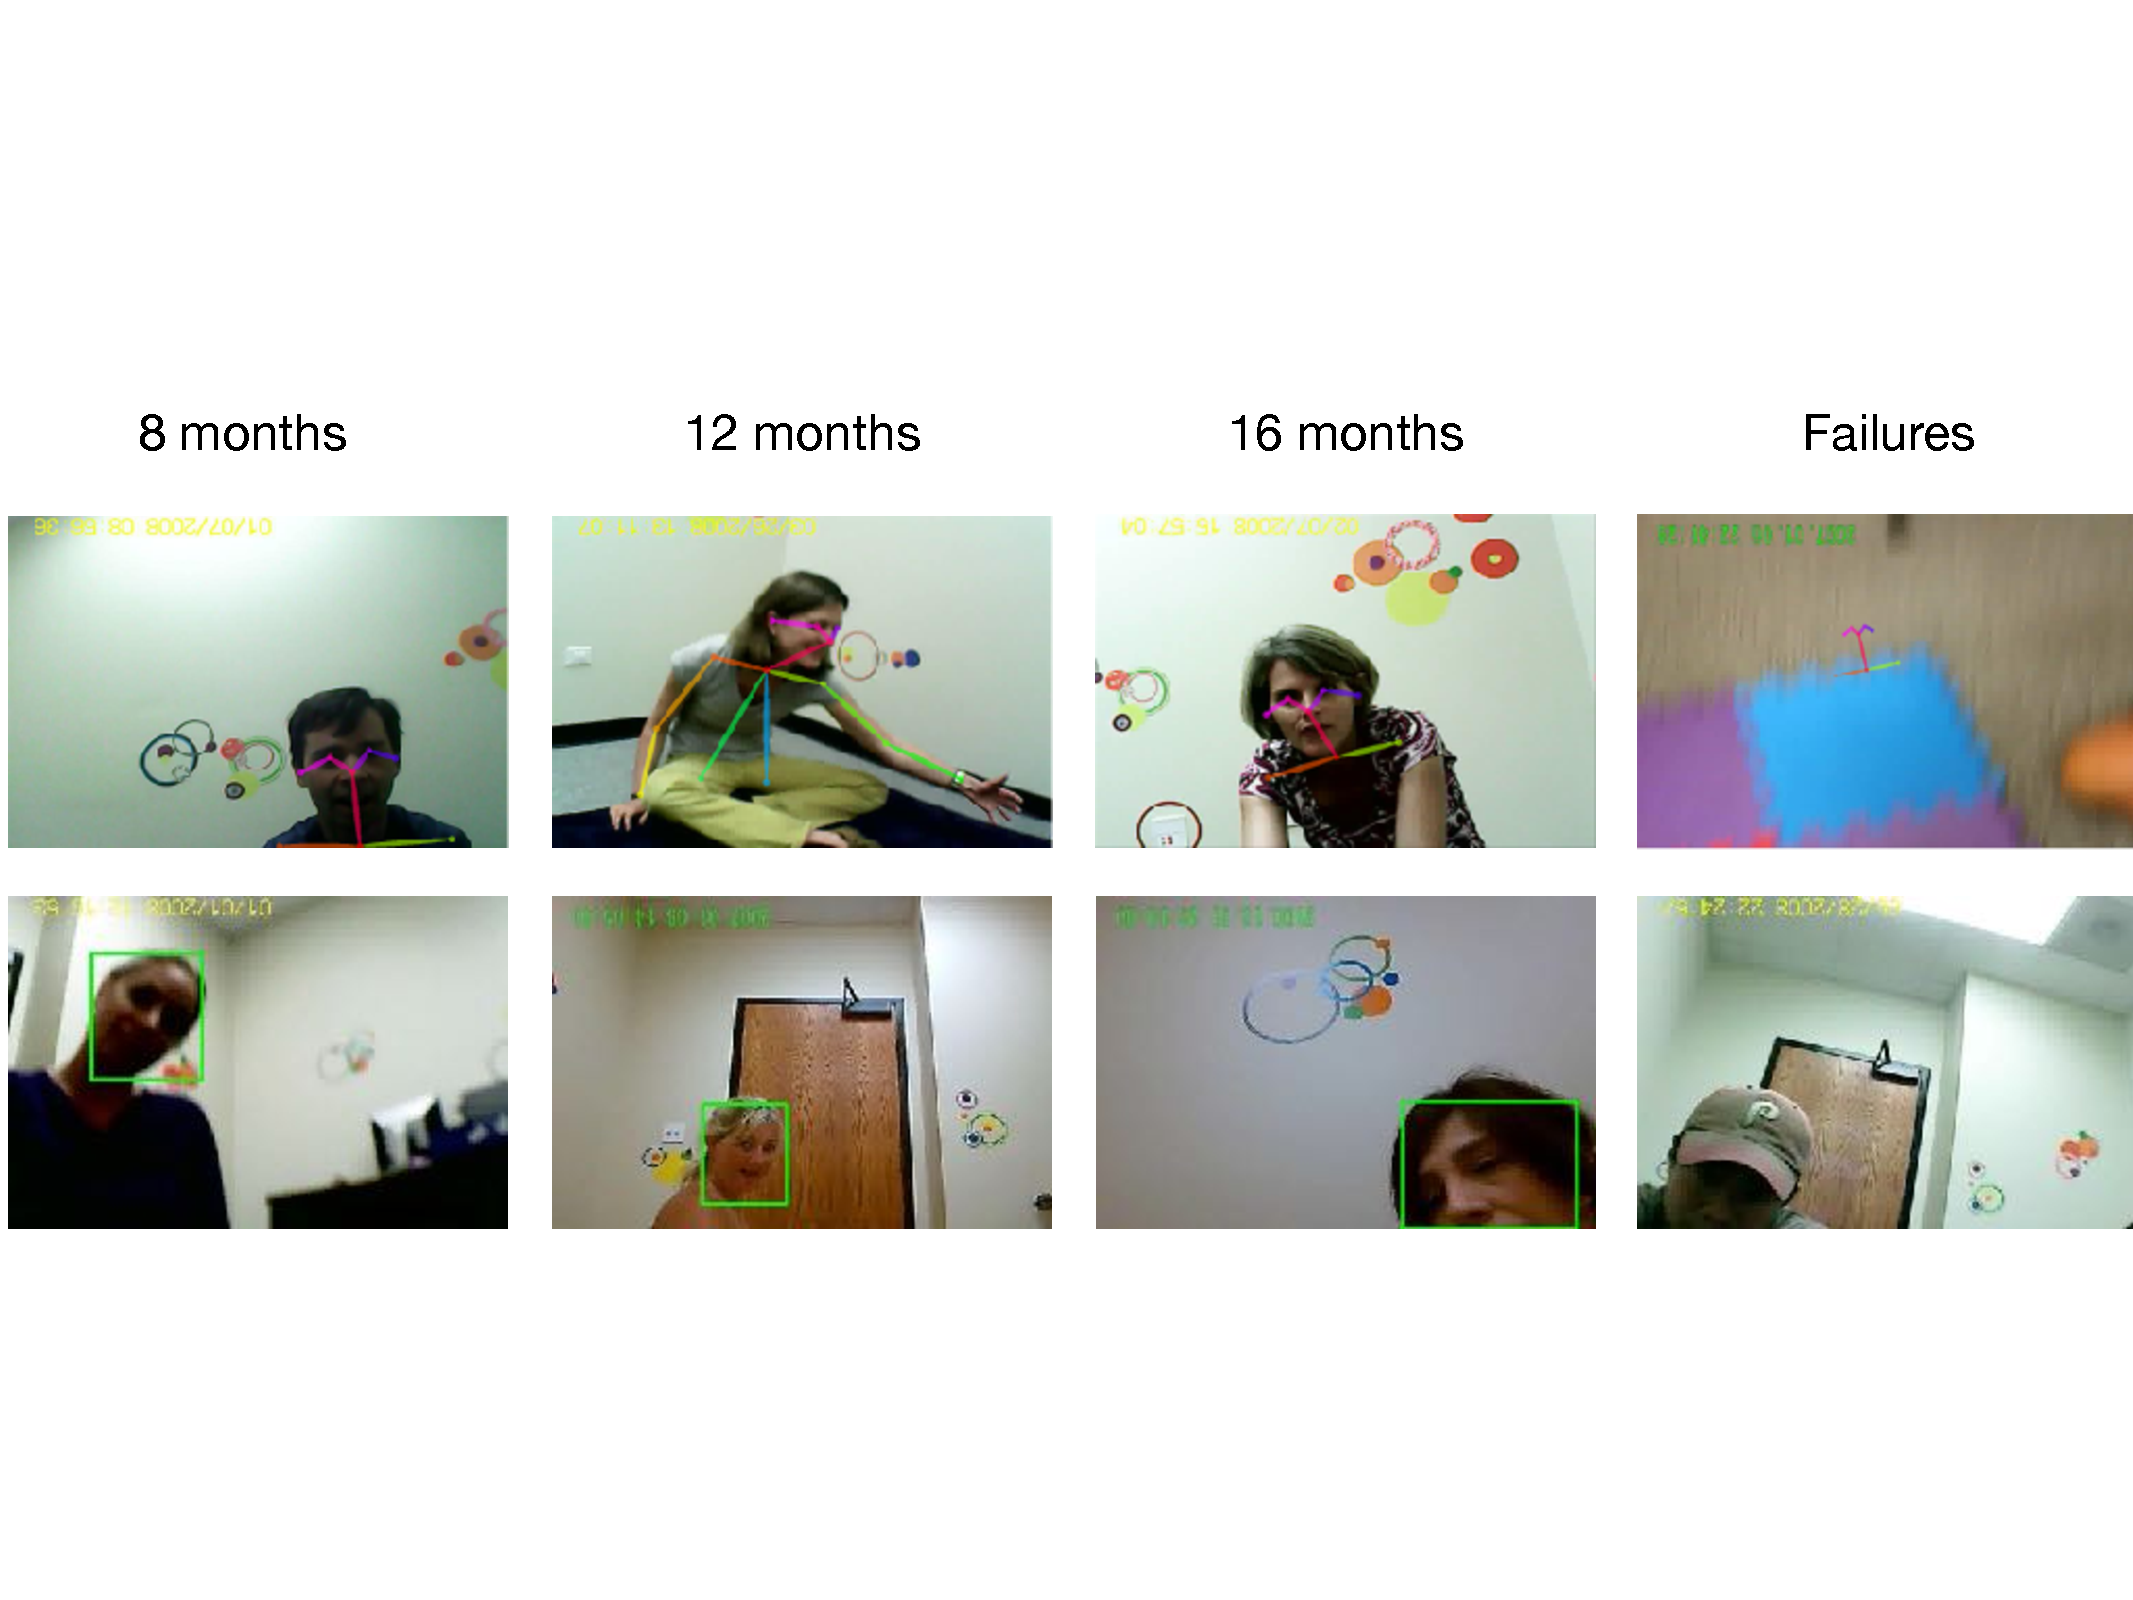
\includegraphics[width=5.5in]{images/detector_samples_banner.pdf}
\caption{\label{fig:frames} Example face and pose detections made by OpenPose (top row) and MTCNN (bottom row) from a child in each age group. The last column features a false positive from OpenPose and a false negative from MTCNN.}
\end{figure*}

\subsubsection{Algorithms}\label{algorithms}

The first face detection system made use of a series of Haar
feature-based cascade classifiers (Viola \& Jones, 2004) applied to each
individual frame. The second algorithm (based on work by K. Zhang et al.
(2016)) uses multi-task cascaded convolutional neural networks (MTCNNs)
for joint face detection and alignment, built to perform well in
real-world environments where varying illuminations and occlusions are
present. We used a Tensorflow implementation of this algorithm avaliable
at \url{https://github.com/davidsandberg/facenet}.

The CNN-based pose detector (OpenPose; Cao et al., 2017; Simon, Joo,
Matthews, \& Sheikh, 2017; Wei, Ramakrishna, Kanade, \& Sheikh, 2016)
provided the locations of 18 body parts (ears, nose, wrists, etc.) and
is available at
\url{https://github.com/CMU-Perceptual-Computing-Lab/openpose}. The
system uses a CNN for initial anatomical detection and subsequently
applies part affinity fields (PAFs) for part association, producing a
series of body part candidates. The candidates are then matched to a
single individual and finally assembled into a pose; here, we only made
use of the body parts relevant to the face and hands (nose and wrists).

\subsubsection{Detector evaluation}\label{detector-evaluation}

To evaluate face detector performance, we hand-labeled a \enquote{gold
set} of labeled frames. To account for the relatively rare appearance of
faces in the dataset, we hand-labeled two types of samples: a sample
containing a high density of faces (half reported by MTCNN, half by
OpenPose) and a random sample from the remaining frames. Each sample was
comprised of an equal number of frames taken from each child's video.
For wrist detections, the \enquote{gold set} was constructed in the same
manner, except frames with a high density of wrists came only from
detections made by OpenPose. Faces were classified as present if at
least half of the face was showing; wrists were classified as present if
any part of the wrist was showing. Two authors labelled the frames
independently and resolved disagreements on a case-by-case basis.
Precision (hits / hits + false alarms), recall (hits / hits + misses),
and F-score (harmonic mean of precision and recall) were calculated for
all detectors and are reported in Table 1.

For face detection, MTCNN outperformed OpenPose when taking into account
only the composite F-score (0.89 MTCNN vs.~0.83 OpenPose). Although
MTCNN and OpenPose performed comparably with the random sample, MTCNN
performed better on the high density sample (specifically looking at
precision), suggesting that OpenPose generated more false positives than
MTCNN. ViolaJones performed quite poorly relative to the other
detectors, especially with respect to the random sample. We thus use
MTCNN detections in the following analyses. For wrist detection,
OpenPose performed moderately well (F = 0.74) with relatively high
precision but low recall on the randomly sampled frames (see Table 1).
We thus analyze wrist detections, with the caveat that we are likely
underestimating the proportion of hands in the dataset.

\begin{table}[ht]
\centering
\begin{tabular}{rllrrr}
\hline
Algorithm & Sample\ Type & P & R & F \\ 
\hline
MTCNN-Faces & High density & 0.89 & 0.92 & \textbf{0.90} \\ 
MTCNN-Faces & Random & 0.94 & 0.62 & 0.75 \\ 
OpenPose-Faces & High density & 0.78 & 0.93 & 0.84 \\ 
OpenPose-Faces & Random & 0.72 & 0.80 & \textbf{0.76} \\ 
ViolaJones-Faces & High density & 0.96 & 0.44 & 0.60 \\ 
ViolaJones-Faces & Random & 0.44 & 0.38 & 0.41 \\ 
OpenPose-Wrists & High density & 0.66 & 1.00 & 0.79 \\ 
OpenPose-Wrists & Random & 0.88 & 0.29 & 0.44 \\ 
\hline
\end{tabular}
\caption{Detector performance on both high density samples (where proportion of targets detected was high) and random samples (where frames were randomly selected). P, R, and F denote precision, recall, and F-score, respectively. Scores in bold are the highest F-scores for each sample type.} 
\vspace{-1em}
\end{table}

\section{Results}\label{results}

First, we report developmental shifts in infants' posture and their
orientation relative to their caregiver, consistent with previous
literature ({\textbf{???}}, {\textbf{???}}). Then, we examine how these
changes influence children's visual access to faces and wrists/hands
across this developmental time range, examining the relative
contributions of age vs.~postural developments. We also explore how
these changes impact the accessibility of faces and wrists/hands during
labeling events, both when parents were labeling familiar objects (e.g.,
\enquote{cat}) as well as novel objects (e.g., \enquote{zem}). Finally,
we apply the same automated detection method to a egocentric video
dataset collected by a different lab ({\textbf{???}}) during which
children's in-the-moment posture was annotated, replicating their
existing results and finding converging support across methods, labs,
and paradigms for the impact of postural developments on children's
visual access to social information.

\begin{figure*}[h]

{\centering \includegraphics{figs/posture-1} 

}

\caption{Proportion of time spent by each infant in different postures and orientations relative to their caregivers (CG); times where posture was not codable are ommitted for visualization purposes}\label{fig:posture}
\end{figure*}

\begin{figure*}[h]

{\centering \includegraphics{figs/indivPosOrient-1} 

}

\caption{Proportion of time spent by each infant in different postures and orientations relative to their caregivers (CG); times where posture was not codable are ommitted for visualization purposes}\label{fig:indivPosOrient}
\end{figure*}

\subsection{Changes in Posture and
Orientation}\label{changes-in-posture-and-orientation}

How do childen's in-the-moment posture and orientation change across
age? In our dataset, the proportion of time infants spent sitting
decreased with age, and the proportion of time infants spent standing
increased with infants' age. As children got older, their locomotive
abilities allowed them to become more independent. Both 8-month-olds and
12-month-olds spent relatively equivalent amounts of time lying/crawling
(i.e., \enquote{prone}) which was markedly decreased in the
16-month-olds, who spent most of their time sitting or standing (see
Figure \ref{fig:posture}). We also observed changes in children's
orientation relative to their caregivers: the 8-month-olds spent more
time with their caregiver behind them supporting their sitting positions
than did children at other ages (see Figure \ref{fig:posture}). However,
we also saw considerable variability across children: some infants spent
almost their entire time sitting at a close distance from their
caregiver, whereas others showed more considerable variability (see
Figure \ref{fig:indivPosOrient}).

\subsection{Changes in Access to Faces and
Hands}\label{changes-in-access-to-faces-and-hands}

We first examined the proportion of face and hand detections as a
function of children's age without considering their posture (see Figure
\ref{fig:detByAge}). While faces tended to be in the field-of-view
overall more often than hands, children's head-mounted cameras were
angled slightly upward to capture the presence of faces, and hand
detections suffered from somewhat lower recall than face detections.
Going forward, we thus analyze differences in the relative proportion of
faces or hands in view as a function of age, posture, and orientation,
rather than comparing them directly. Overall, we observed that
12-month-olds appeared to have visual access to slightly fewer faces
than 8 or 16-month-olds, creating a slight U-shaped function in face
detections; conversely, hand detections were showed a slight increase
across this age range, as reported in prior literature ({\textbf{???}}).

However, these age-related trends were much smaller than the effect of
infant's postural developments on children's visual access to faces and
hands. Children's in-the-moment posture was a major factor both in how
many faces and hands were in view during the play session, as was their
orientation relative to their caregiver. Infants who were sitting or
standing had more faces in view than infants who were lying
down/crawling (i.e.~prone), which was most frequent among 12-month-olds
relative to the other age groups (Figure \ref{fig:detByPosOrient}). When
caregivers were behind their children, supporting their children's
sitting or standing positions, children saw fewer faces and wrists. In
particular, children who were sitting or in front of their caregiver had
a high proportion of faces and hands in their field of view. (Figure
\ref{fig:detByPosOrient}, lower panel).

These trends were quantified using two generalized linear mixed-effect
models estimating the proportion of faces and hands that were in view,
with orientation, posture, their interaction, and scaled participant's
age as fixed effects, and with random slopes for infants' orientation
and posture. A summary of the coefficients of the models can be found in
Table 2, confirming that infants who were sitting/standing and in front
of their caregivers saw the most faces and hands. When modeling the
proportion of faces seen, age was not a significant predictor; however,
age remained a significant predictor when modeling the proportion of
hands seen by infants. Overall, these results suggest that infants'
visual access to social information is largely modulated by their
posture and orientation to their caregiver, which is in turn a function
of their general locomotor development. Nonetheless, these results also
suggest that infants may still increase their attention to hands
throughout this age range as they continue to learn about objects, their
functions, and their names.

\subsection{Access to Faces and Hands During Labeling
Events}\label{access-to-faces-and-hands-during-labeling-events}

Our play session was designed to provide parents with opporunities to
label objects--both familiar and novel--such that we could examine
whether children seek out different kinds of social information around
naming events. We thus explored how face and hand detections changed
during object labeling events, analyzing a four-second window around
each labeling event (e.g., \enquote{Look at the {[}zem{]}!}). Every
utterance of one of the labelled objects (e.g., \enquote{ball}) was
counted as a \enquote{labeling event}; timestamps of the beginning of
each word were hand-annotated from transcripts ad synchronized with the
frame-by-frame detections. Overall, we did not find major differences in
face/hand detections during naming events relative to baseline, either
for novel objects or for familiar objects (see Figure
\ref{fig:detByNaming}). This was true both when we analyzed naming rates
with or without taking into account children's posture and orientation
relative to their caregiver. These results suggest that either children
did not actively seek out social information during this particular play
session around naming events, perhaps because were a limited number of
possible referents at any given time.

\begin{figure*}[h]

{\centering \includegraphics{figs/detByAge-1} 

}

\caption{Proportion of faces (left) and wrists (right) detected by the OpenPose model as a function of child's age. Larger dots indicate children who had longer play sessions and thus for whom there was more data.}\label{fig:detByAge}
\end{figure*}

\begin{figure*}[h]

{\centering \includegraphics{figs/detByPosOrient-1} 

}

\caption{Proportion of face / wrist detections by children's age, their posture, and their caregivers orientation. Data points are scaled by the amount of time spent in each orientation/posture combination; times when posture/orientation annotatinos were unavaliable or the infant was carried are not plotted. Error bars represent 95\% bootstrapped confidence intervals}\label{fig:detByPosOrient}
\end{figure*}

\begin{figure*}[h]

{\centering \includegraphics{figs/detByNaming-1} 

}

\caption{Proportion of face / wrist detections during naming events (+/- 2 seconds around label)for familiar and novel objects; these rates are put into context relative to baseline Error bars represent 95\% bootstrapped confidence intervals.}\label{fig:detByNaming}
\end{figure*}

\section{Extension to Franchak et al.,
2017}\label{extension-to-franchak-et-al.-2017}

In the present work, we found that infant's in-the-moment posture
changed with their age, as did infants' orientation relative their
caregiver. In a related study with 12-month-olds, ({\textbf{???}}) also
that children's in-the-moment posture changed the amount of time infants
spent looking at faces. Here, we sought to replicate the findings from
({\textbf{???}}) using our automated methodology (OpenPose detections),
using the footage from their head-mounted cameras (shared on Databrary,
({\textbf{???}})).

This dataset differed from the present in two key ways that could
present a challenge for our automated methodology. First, the
environment that infants were immersed in with their caregivers (and
experimenters) was much larger and more varied than the play room used
in the present dataset, containing multiple structures and toys in
different parts of the room for infants to explore, unlike the present
room dataset which was relatively small (approximately 10' x 10'). Thus,
our automated methodology could fail to generalize to scenes from these
more complex environments, where detecting faces and hands could
arguably be a much harder task. Second, ({\textbf{???}}) used a
head-mounted eye-tracker, finding that children's posture affected where
children were looking within their visual field. Nonetheless, if
children are often orienting their heads towards where they are
allocating their attention ({\textbf{???}}) then we should expect to
find the same pattern of results only when analyzing the information in
view.

\begin{figure*}[h]

{\centering \includegraphics{figs/franchak-1} 

}

\caption{Proportion of face / wrist detections for 12-month-olds in Franchak et al., 2017 as a function of children's in-the-moment posture. Error bars represent 95 percent bootstrapped confidence intervals.}\label{fig:franchak}
\end{figure*}

Overall, we found convergence between our two methodologies: we
replicated ({\textbf{???}})\enquote{s main results, finding that the
proportion of faces in view was greater when infants were sitting or
standing vs.~prone. We also found the same patterns of results with
hands (i.e., wrist detectinos), which were not originally annotated in
({\textbf{???}}) (see Figure \ref{fig:franchak}); results were validated
with generalized mixed effect models as in our previous analysis.
Interestingly, there was a relatively higher proportion of hands in view
in ({\textbf{???}}) relative to the present dataset; this is likely
mostly due to the fact that there were often multiple people in view:
experimenters stayed in the room to film children and assist with
technical difficulties, while in our present dataset the experiments
left the room for the majority of the play session. Nonetheless, we
still found that posture modulated the hands in view as well, suggesting
that this is a major factor that structures infants} access to visual
information.

\section{Discussion}\label{discussion}

\section{Discussion}\label{discussion-1}

\newpage

\section{References}\label{references}

\begingroup
\setlength{\parindent}{-0.5in} \setlength{\leftskip}{0.5in}

\hypertarget{refs}{}
\hypertarget{ref-adolph2006motor}{}
Adolph, K. E., \& Berger, S. E. (2006). Motor development.
\emph{Handbook of Child Psychology}.

\hypertarget{ref-adolph2012toward}{}
Adolph, K. E., Gilmore, R. O., Freeman, C., Sanderson, P., \& Millman,
D. (2012). Toward open behavioral science. \emph{Psychological Inquiry},
\emph{23}(3), 244--247.

\hypertarget{ref-bambach2017}{}
Bambach, S., Crandall, D. J., Smith, L. B., \& Yu, C. (2017). An
egocentric perspective on active vision and visual object learning in
toddlers. In \emph{Proceedings of the seventh joint ieee conference on
development and learning and on epigenetic robotics}.

\hypertarget{ref-brooks2005}{}
Brooks, R., \& Meltzoff, A. (2005). The development of gaze following
and its relation to language. \emph{Developmental Science}, \emph{8}(6),
535--543.

\hypertarget{ref-brooks2008}{}
Brooks, R., \& Meltzoff, A. N. (2008). Infant gaze following and
pointing predict accelerated vocabulary growth through two years of age:
A longitudinal, growth curve modeling study. \emph{Journal of Child
Language}, \emph{35}(1), 207--220.

\hypertarget{ref-cao2017realtime}{}
Cao, Z., Simon, T., Wei, S.-E., \& Sheikh, Y. (2017). Realtime
multi-person 2D pose estimation using part affinity fields. In
\emph{CVPR}.

\hypertarget{ref-carpenter1998}{}
Carpenter, M., Nagell, K., \& Tomasello, M. (1998). Social cognition,
joint attention, and communicative competence from 9 to 15 months of
age. \emph{Monographs of the Society for Research in Child Development},
\emph{63}(4).

\hypertarget{ref-clerkin2017}{}
Clerkin, E. M., Hart, E., Rehg, J. M., Yu, C., \& Smith, L. B. (2017).
Real-world visual statistics and infants' first-learned object names.
\emph{Phil. Trans. R. Soc. B}, \emph{372}(1711), 20160055.

\hypertarget{ref-farroni2002eye}{}
Farroni, T., Csibra, G., Simion, F., \& Johnson, M. H. (2002). Eye
contact detection in humans from birth. \emph{Proceedings of the
National Academy of Sciences}, \emph{99}(14), 9602--9605.

\hypertarget{ref-fausey2016}{}
Fausey, C. M., Jayaraman, S., \& Smith, L. B. (2016). From faces to
hands: Changing visual input in the first two years. \emph{Cognition},
\emph{152}, 101--107.

\hypertarget{ref-franchak2011}{}
Franchak, J. M., Kretch, K. S., Soska, K. C., \& Adolph, K. E. (2011).
Head-mounted eye tracking: A new method to describe infant looking.
\emph{Child Development}, \emph{82}(6), 1738--1750.

\hypertarget{ref-frank2013}{}
Frank, M. C., Simmons, K., Yurovsky, D., \& Pusiol, G. (2013).
Developmental and postural changes in children's visual access to faces.
In \emph{Proceedings of the 35th annual meeting of the cognitive science
society} (pp. 454--459).

\hypertarget{ref-iverson2010}{}
Iverson, J. M. (2010). Developing language in a developing body: The
relationship between motor development and language development.
\emph{Journal of Child Language}, \emph{37}(2), 229--261.

\hypertarget{ref-karasik2014}{}
Karasik, L. B., Tamis-LeMonda, C. S., \& Adolph, K. E. (2014). Crawling
and walking infants elicit different verbal responses from mothers.
\emph{Developmental Science}, \emph{17}(3), 388--395.

\hypertarget{ref-scheirer2014perceptual}{}
Scheirer, W. J., Anthony, S. E., Nakayama, K., \& Cox, D. D. (2014).
Perceptual annotation: Measuring human vision to improve computer
vision. \emph{IEEE Transactions on Pattern Analysis and Machine
Intelligence}, \emph{36}(8), 1679--1686.

\hypertarget{ref-simon2017hand}{}
Simon, T., Joo, H., Matthews, I., \& Sheikh, Y. (2017). Hand keypoint
detection in single images using multiview bootstrapping. In
\emph{CVPR}.

\hypertarget{ref-viola2004robust}{}
Viola, P., \& Jones, M. J. (2004). Robust real-time face detection.
\emph{International Journal of Computer Vision}, \emph{57}(2), 137--154.

\hypertarget{ref-walle2014}{}
Walle, E. A., \& Campos, J. J. (2014). Infant language development is
related to the acquisition of walking. \emph{Developmental Psychology},
\emph{50}(2), 336.

\hypertarget{ref-wei2016cpm}{}
Wei, S.-E., Ramakrishna, V., Kanade, T., \& Sheikh, Y. (2016).
Convolutional pose machines. In \emph{CVPR}.

\hypertarget{ref-yoshida2008}{}
Yoshida, H., \& Smith, L. (2008). What's in view for toddlers? Using a
head camera to study visual experience. \emph{Infancy}, \emph{13},
229--248.

\hypertarget{ref-yurovsky2012}{}
Yurovsky, D., Smith, L., \& Yu, C. (in press). Statistical word learning
at scale: The baby's view is better. \emph{Developmental Science}.

\hypertarget{ref-zhang2016}{}
Zhang, K., Zhang, Z., Li, Z., \& Qiao, Y. (2016). Joint face detection
and alignment using multitask cascaded convolutional networks.
\emph{IEEE Signal Processing Letters}, \emph{23}(10), 1499--1503.

\endgroup

\end{document}
